\providecommand{\main}{../../../..}
\documentclass[\main/dresen_thesis.tex]{subfiles}

\begin{document}
  \label{sec:monolayers:nanoparticle:tem}
  The exemplary TEM micrographs in \reffig{fig:monolayers:nanoparticle:tem} show in all cases nanoparticles with a cubic shape.
  Ol-CoFe-C have an average edge length of $10.90(4) \unit{nm}$ and present the lowest size distribution with $8.8(3) \unit{\%}$.
  Inspecting the nanocubes of Ol-CoFe-C more closely in the micrograph shows for many cubes a round dark core area within the cube.
  For the nanocubes prepared by acetylacetonates such phenomenon is not observed.
  Within Ac-CoFe-C, the size distribution is evaluated to a larger value of $13.9(9) \unit{\%}$ and non-cubic particles can be found among the cubes.
  Their average edge length is estimated to $10.1(1) \unit{nm}$ by the log-normal distribution fit.
  Ac-CoFe-C-2 has an intermediate size distribution of $9.9(8) \%$ and an average edge length of $10.8(1) \unit{nm}$.
  Here, the micrographs reveal additionally to the cubes larger non-cubic particles with an approximate extend of $15 \ldots 20 \unit{nm}$ in between the cubes.
  The third nanoparticle batch from acetylacetonates Ac-CoFe-C-3 is slightly larger with $12.5(1) \unit{nm}$ and has a size distribution of $13.2(9) \%$.
  The values evaluated from TEM are summarized in \reftab{tab:monolayers:nanoparticles:discussion:tem}.

  In direct comparison of the TEM micrographs, the particles synthesized from cobalt/iron oleates (Ol-CoFe-C) are qualitatively the most homogeneous in shape.
  The oleate synthesis can therefore be considered as the better route in contrast to the synthesis from acetylacetonates  if only a homogeneous shape and small size distribution for the nanoparticles is the criterion.
  The darker core area for Ol-CoFe-C is in agreement with the literature reports of a core-shell structure for nanocubes prepared from metal oleates in 1-octadecene \cite{Bao_2009_Forma, Bodnarchuk_2009_Excha, Wetterskog_2013_Anoma}.

  \begin{figure}[tb]
    \centering
    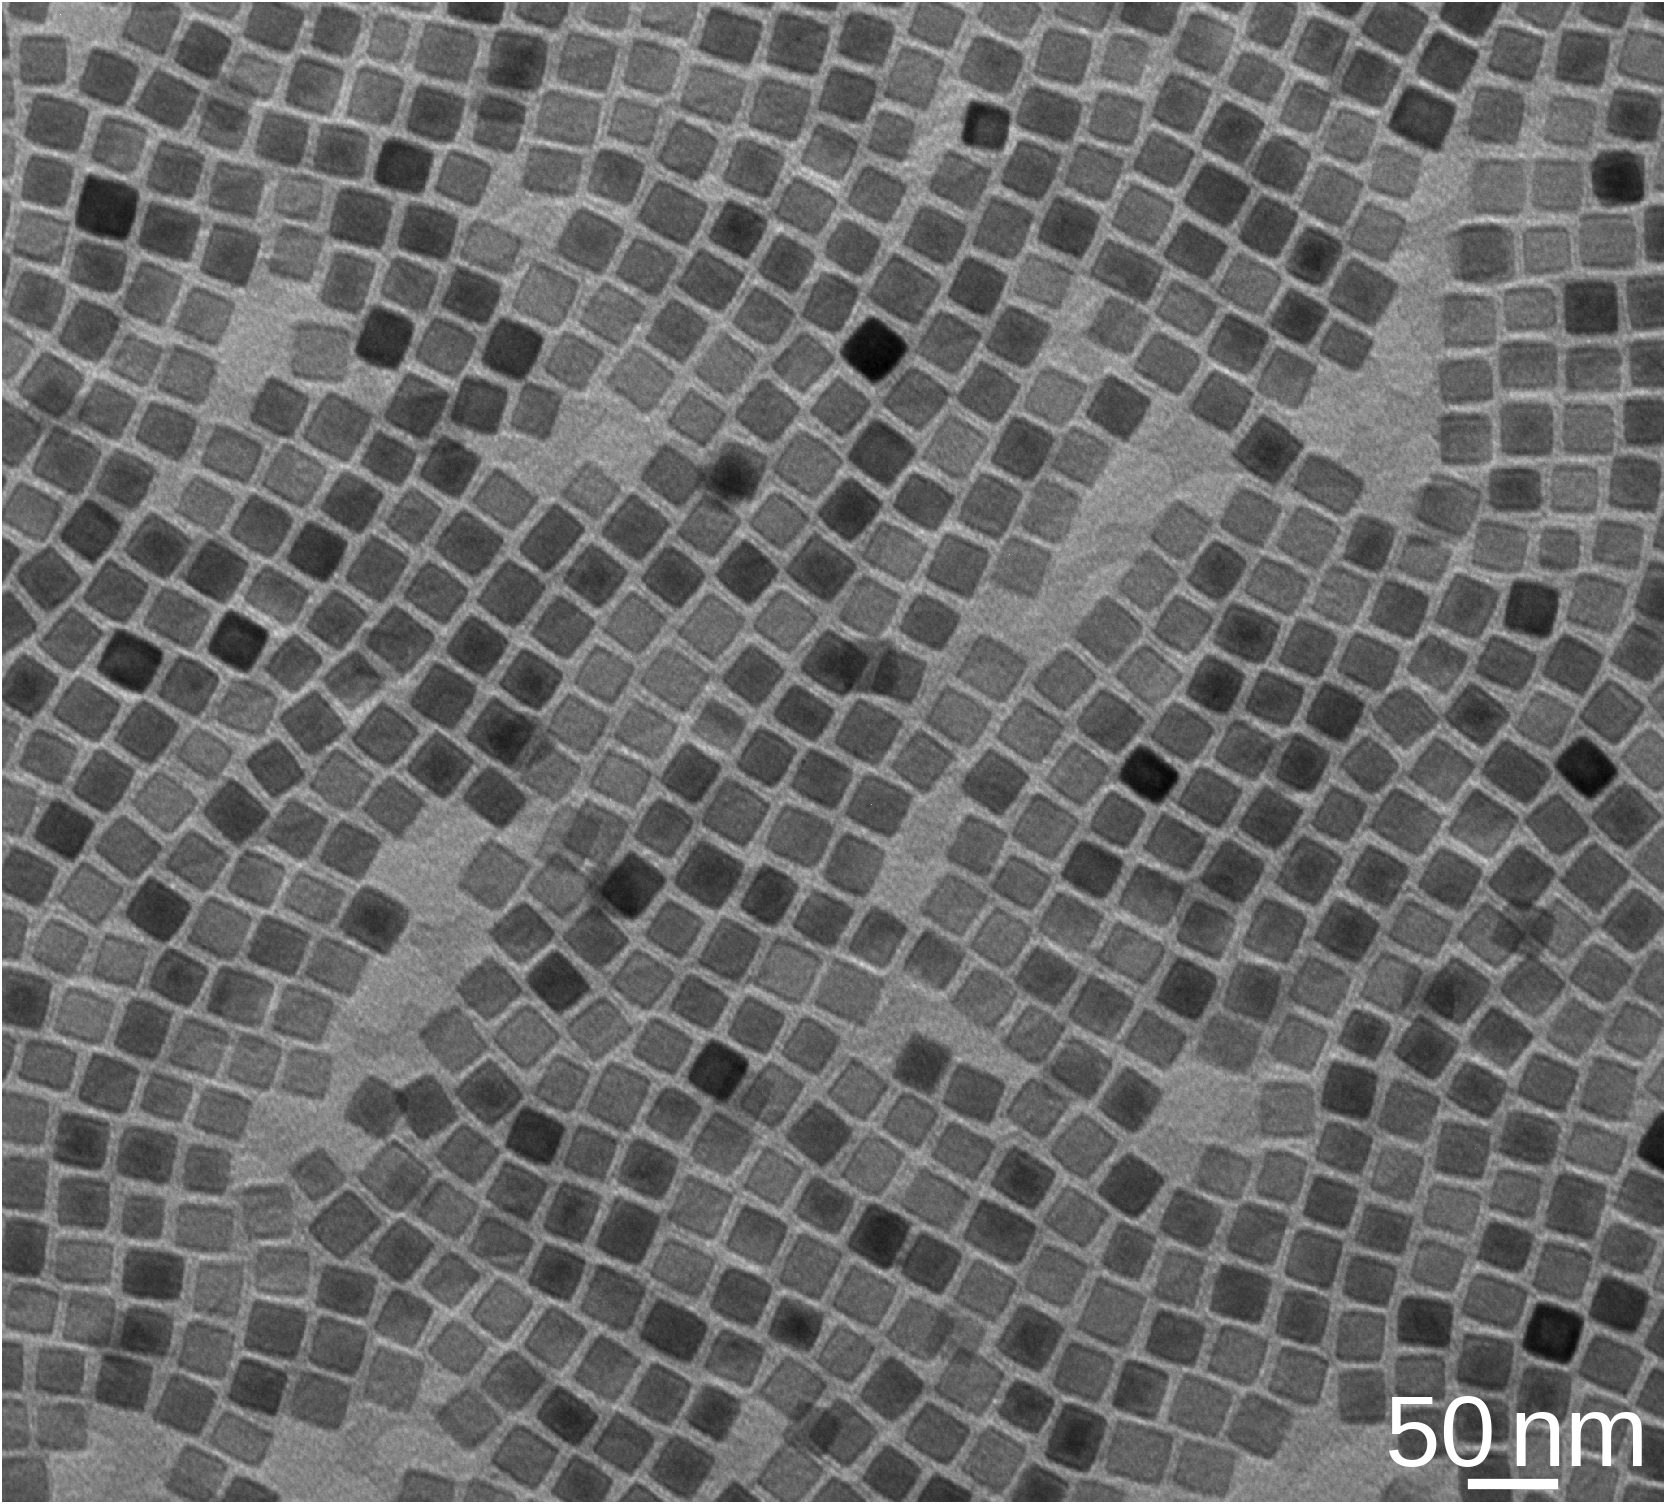
\includegraphics{monolayers_TEM_Ol_CoFe_C}
    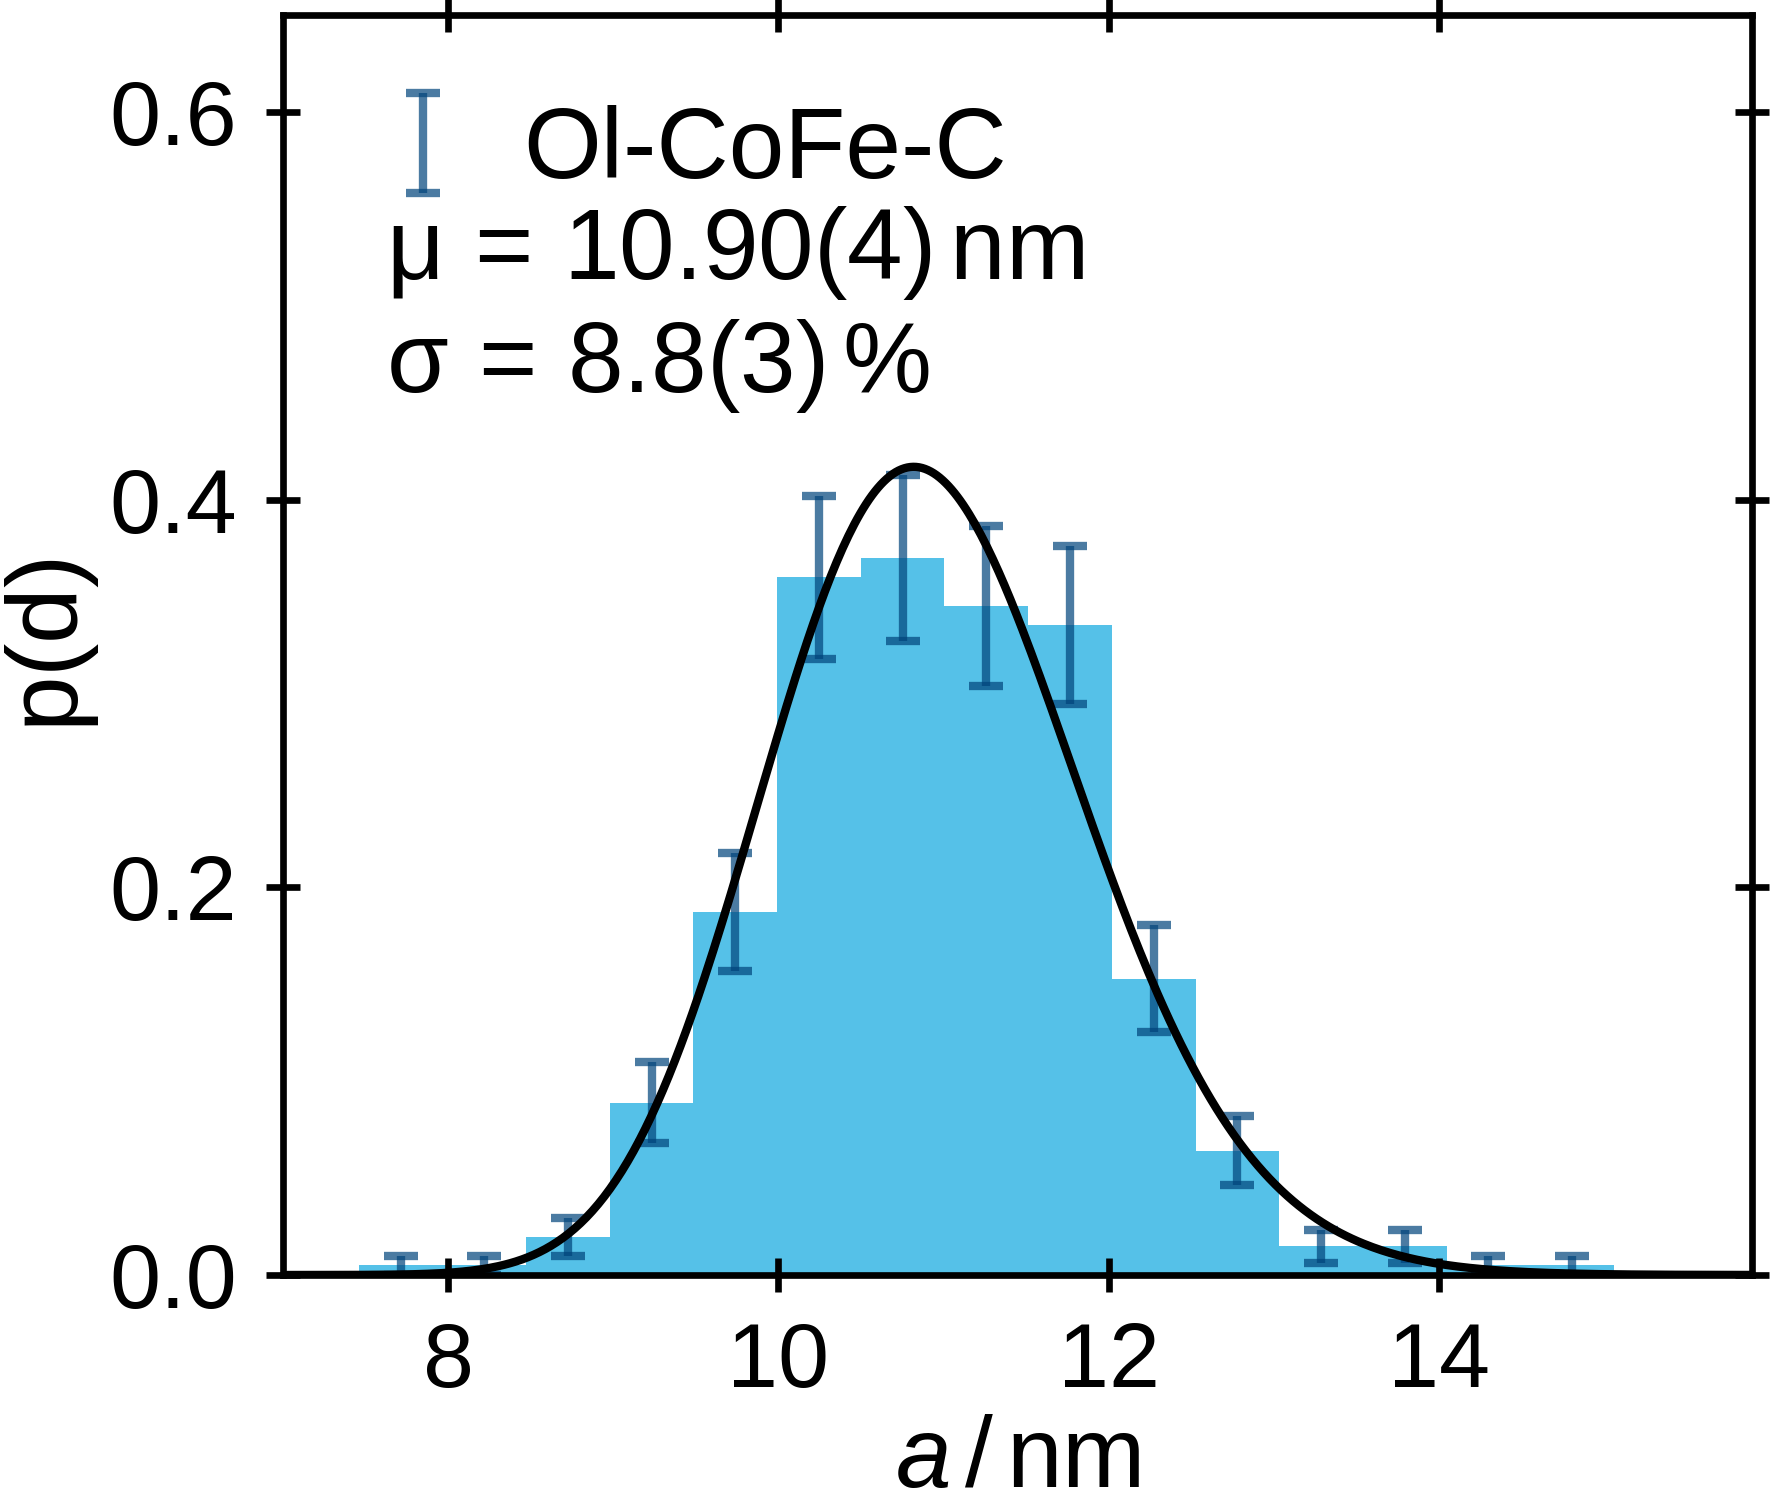
\includegraphics{monolayers_TEM_Ol_CoFe_C_sizeDist}
    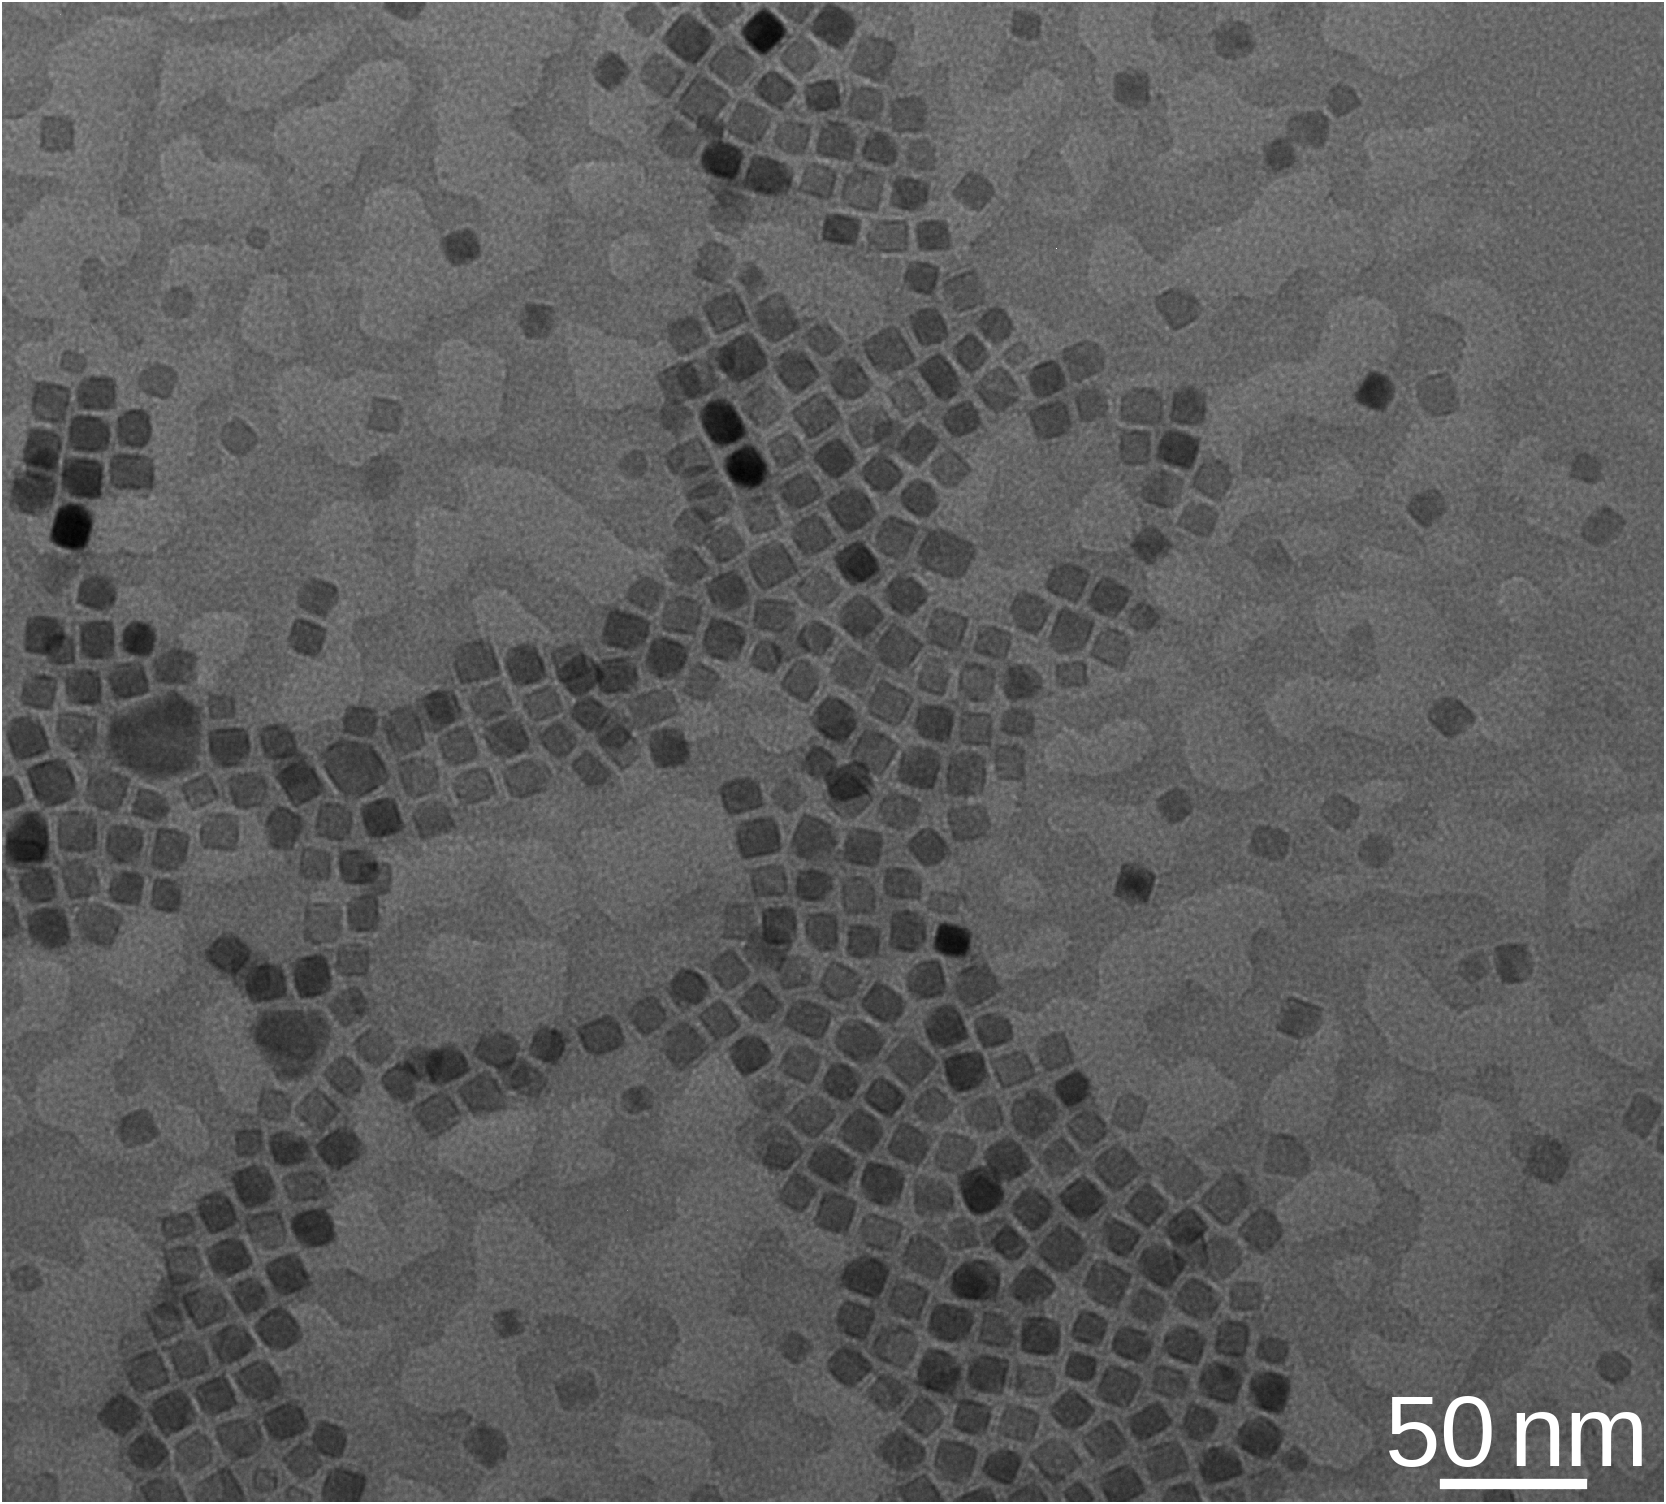
\includegraphics{monolayers_TEM_Ac_CoFe_C}
    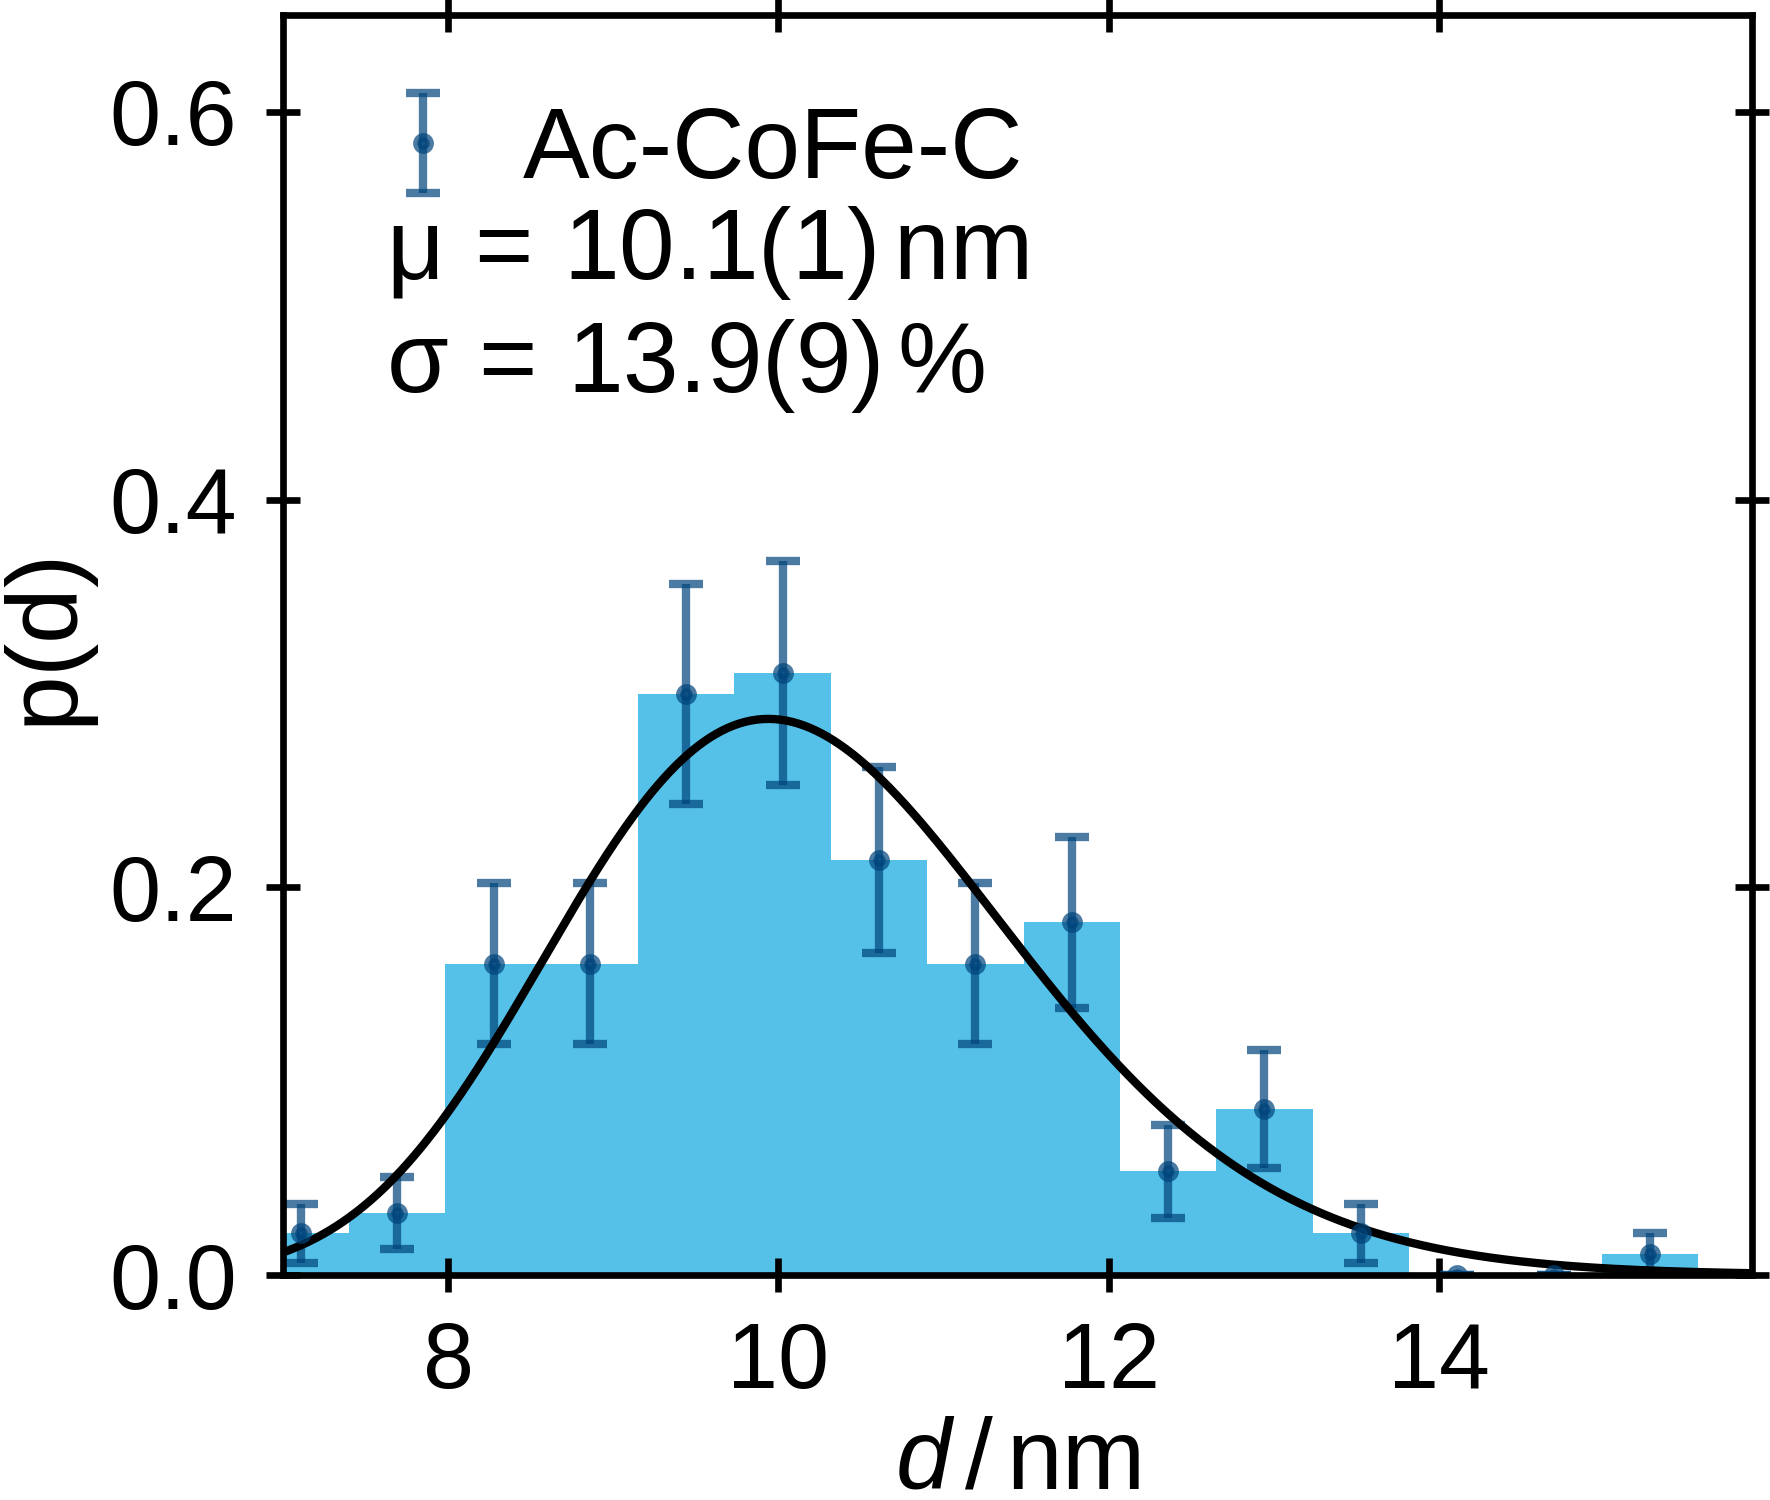
\includegraphics{monolayers_TEM_Ac_CoFe_C_sizeDist}
    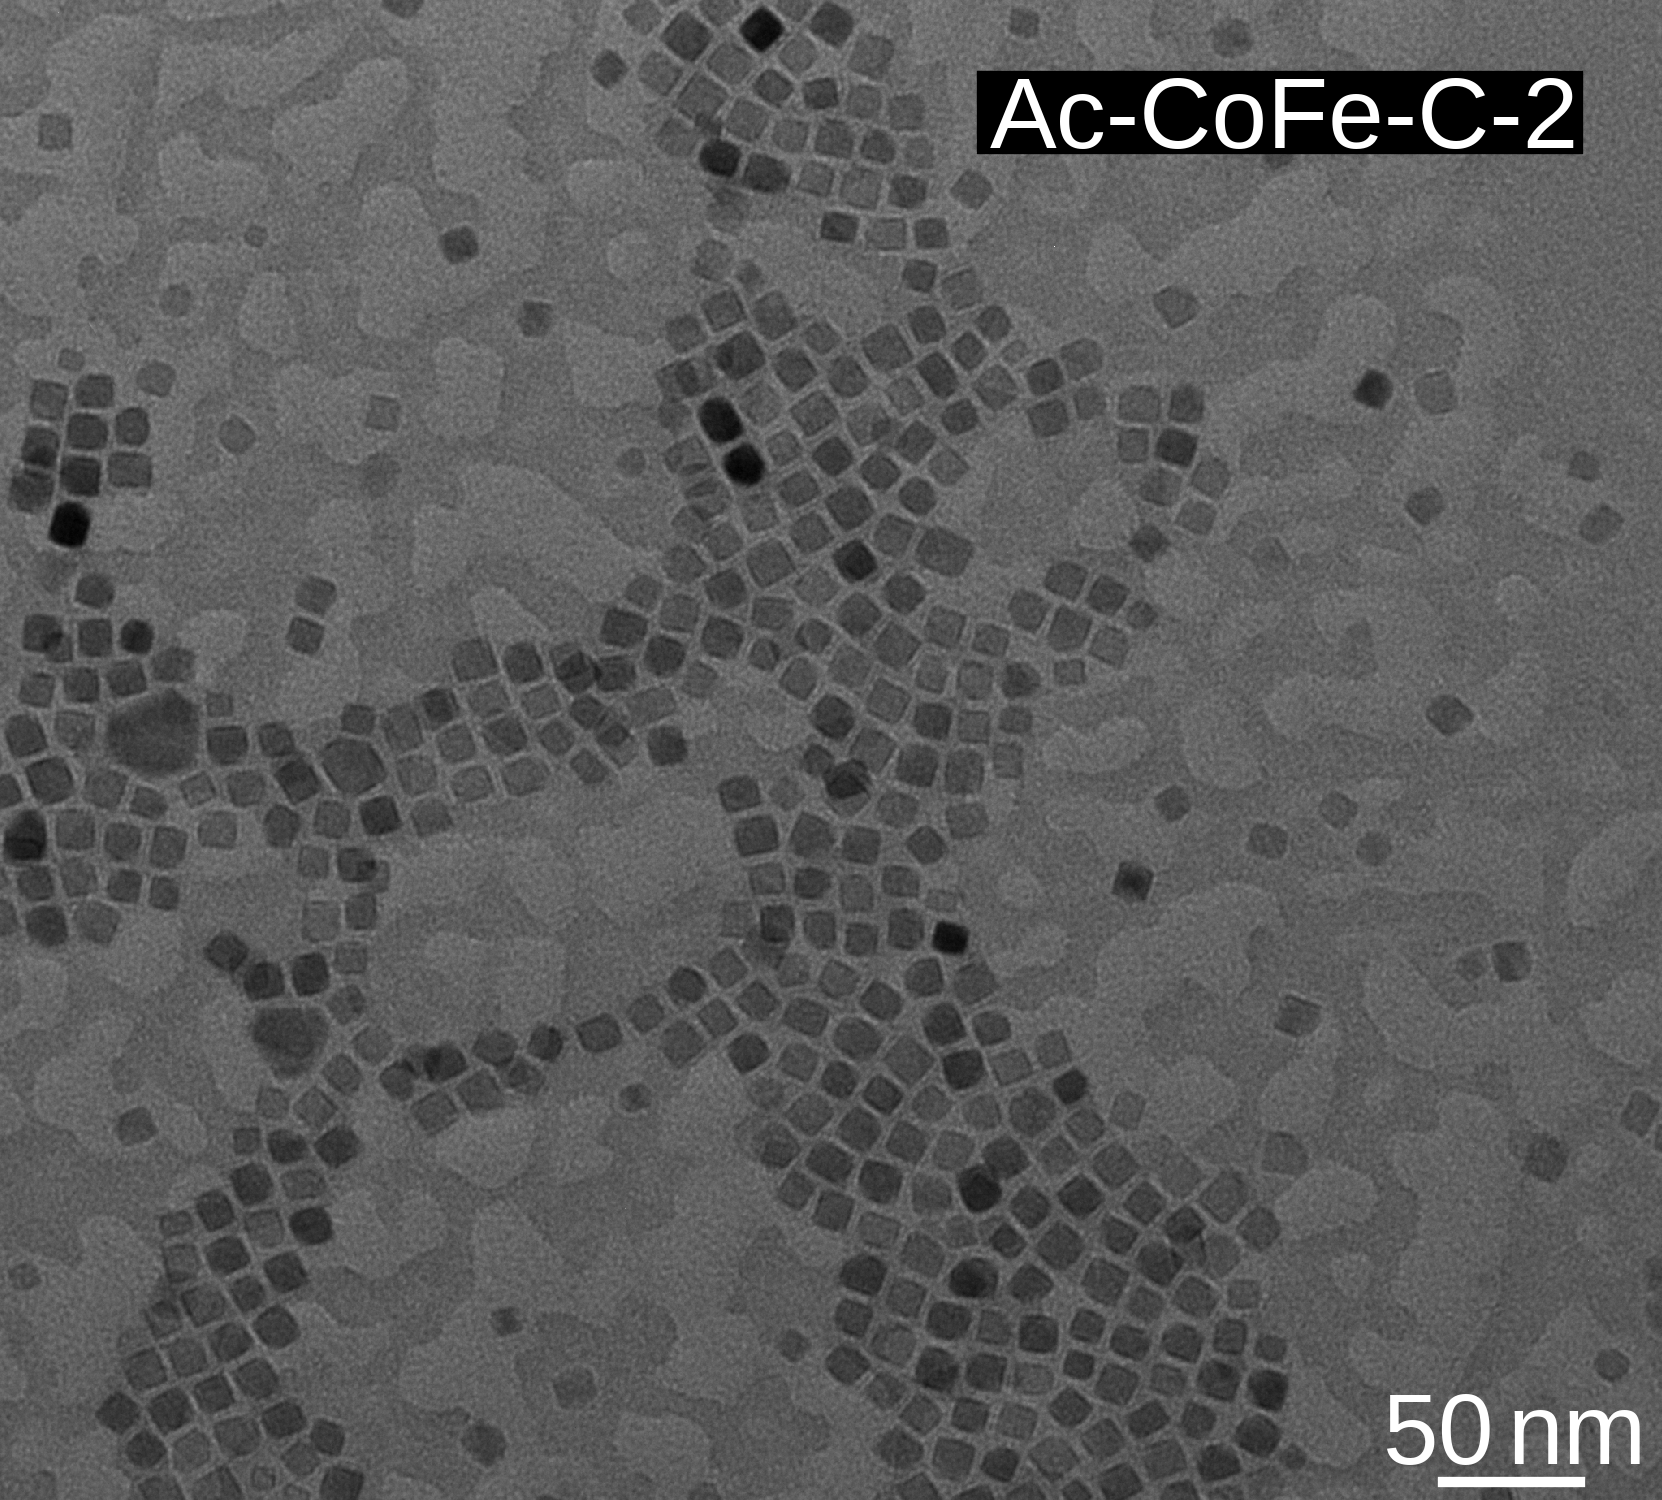
\includegraphics{monolayers_TEM_Ac_CoFe_C_2}
    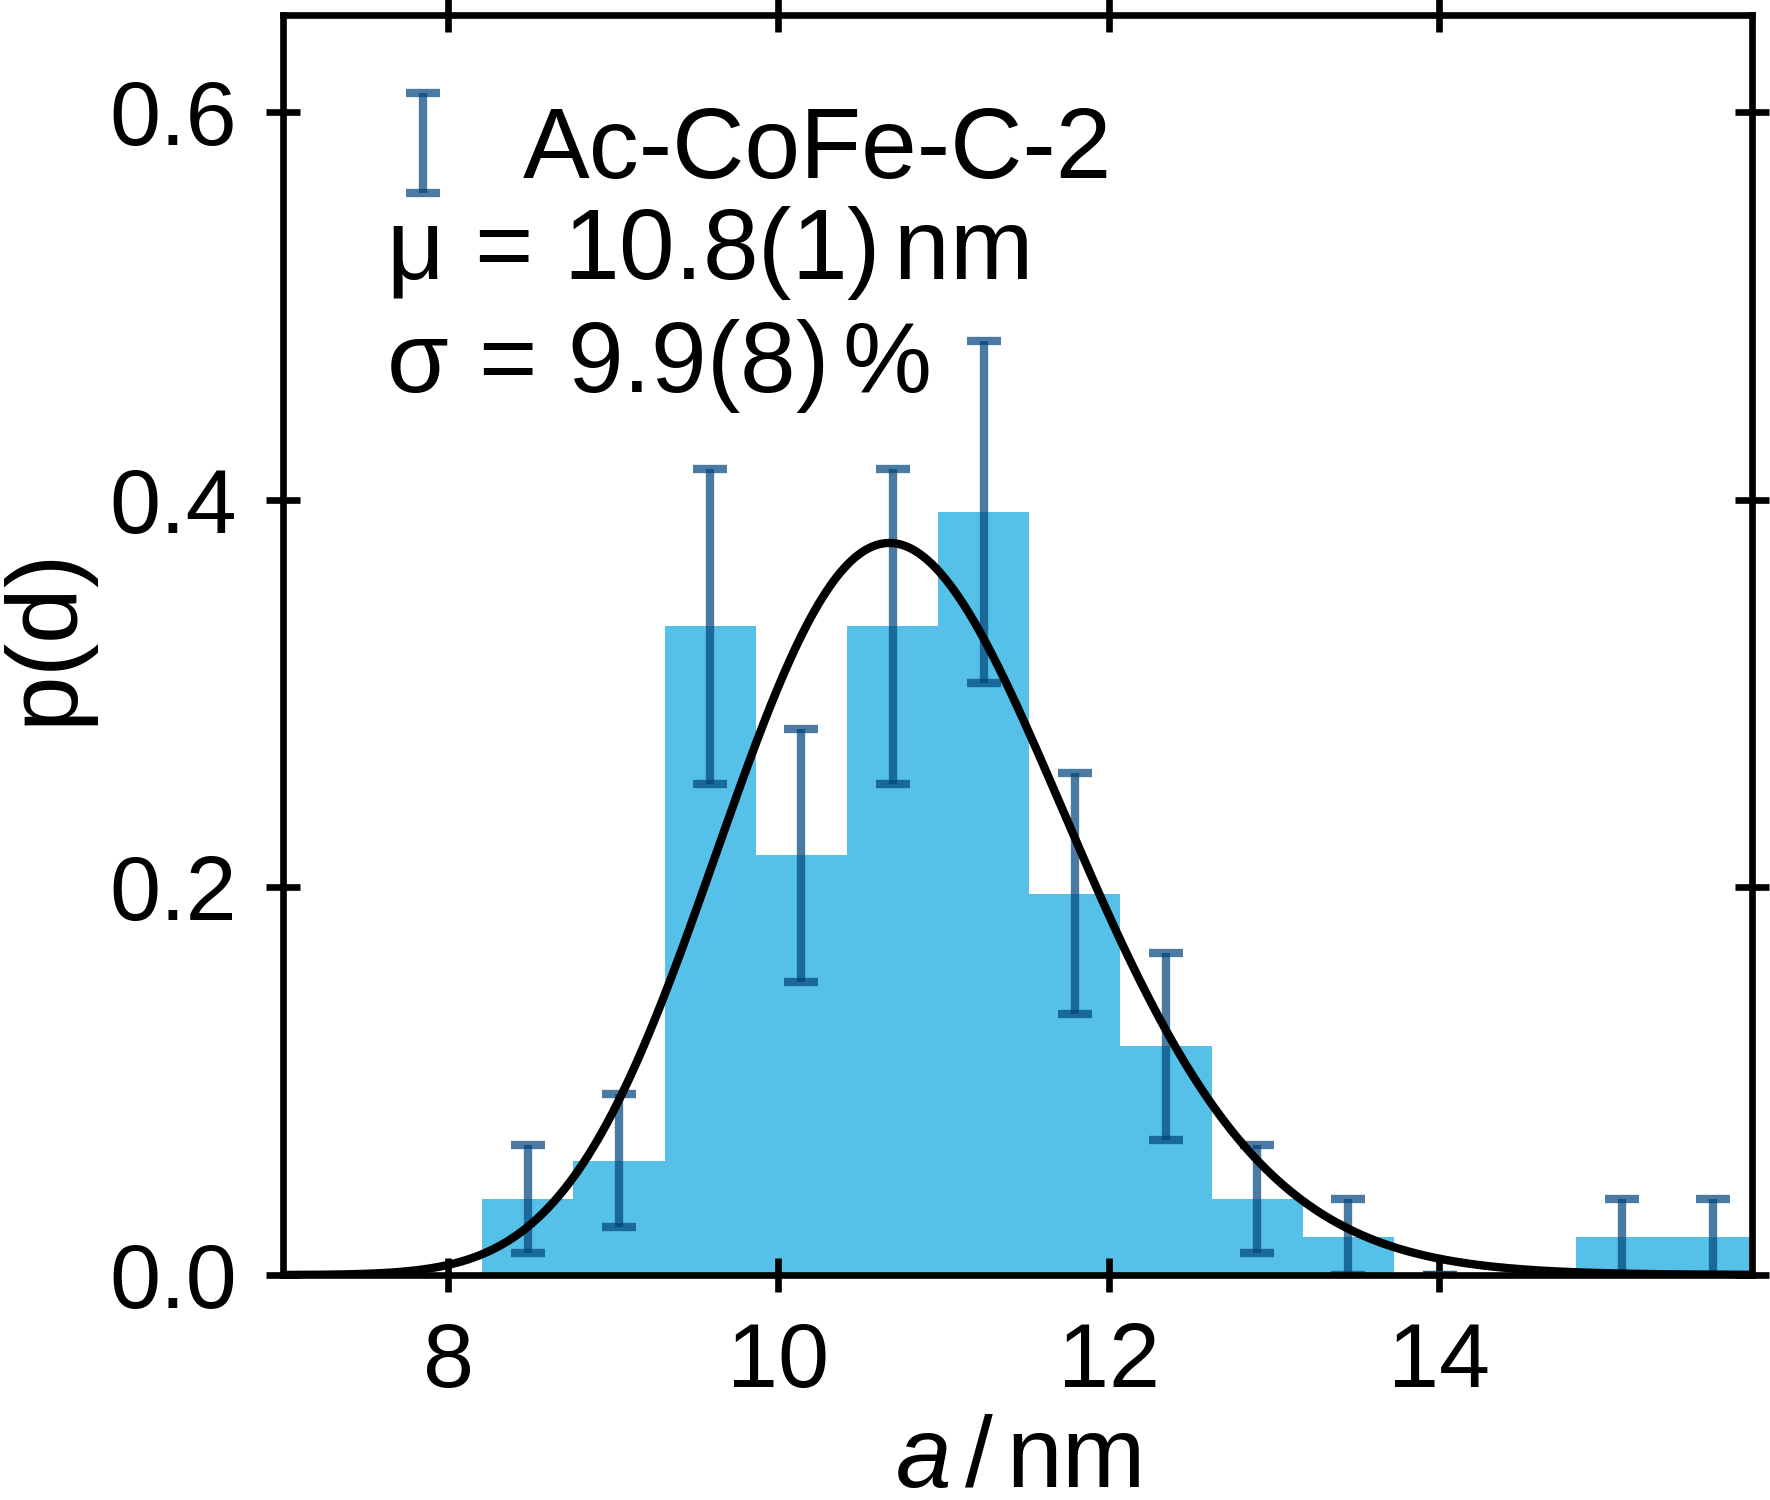
\includegraphics{monolayers_TEM_Ac_CoFe_C_2_sizeDist}
    \caption{\label{fig:monolayers:nanoparticle:tem}Bright field TEM micrographs (left) and evaluated size distribution (right) of the nanoparticle batches Ol-CoFe-C (upper), Ac-CoFe-C (center) and Ac-CoFe-C-2 (lower).}
  \end{figure}
  \begin{figure}[tb]
    \centering
    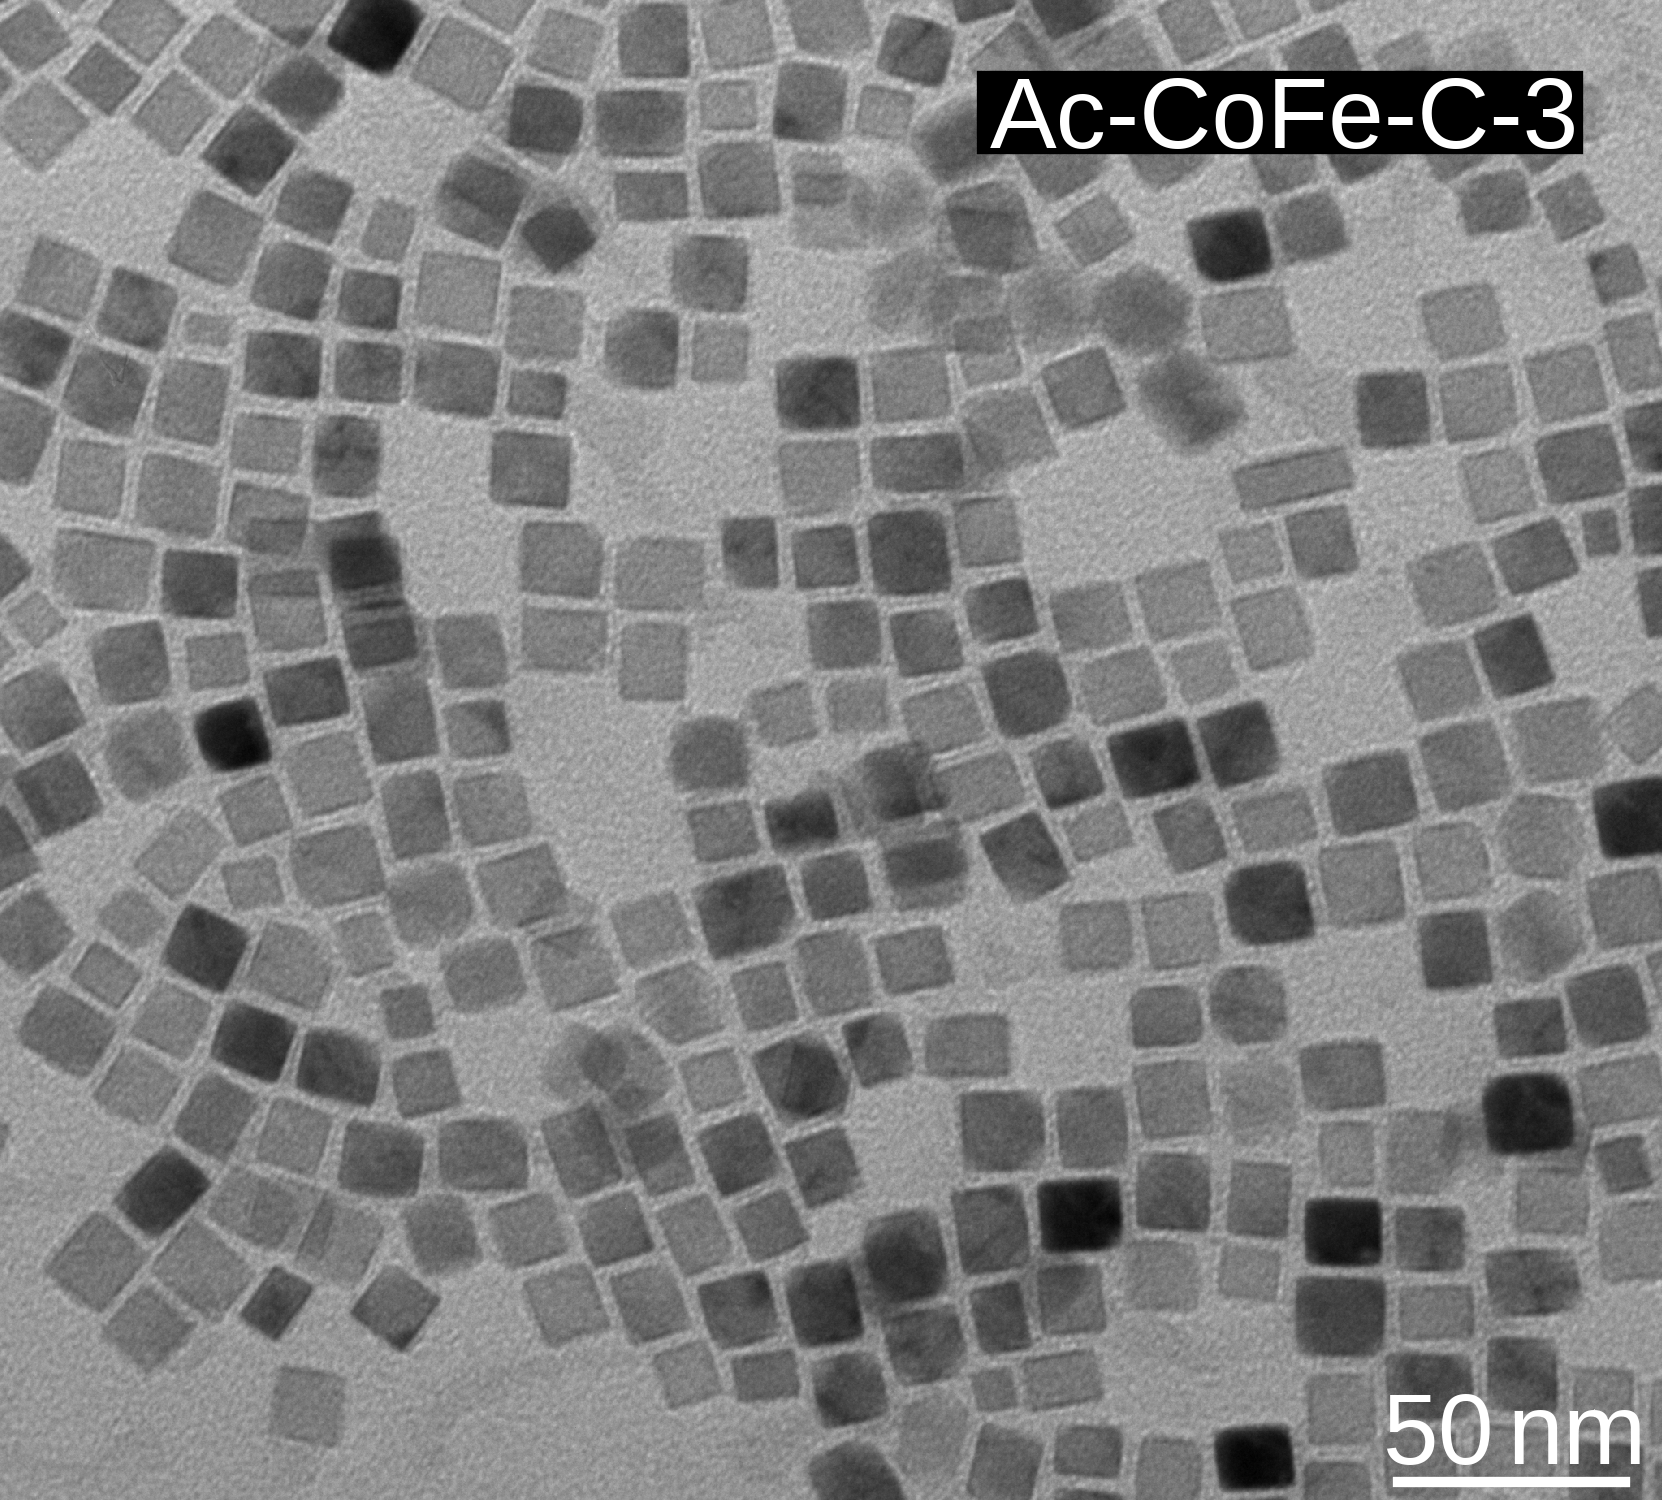
\includegraphics{monolayers_TEM_Ac_CoFe_C_3}
    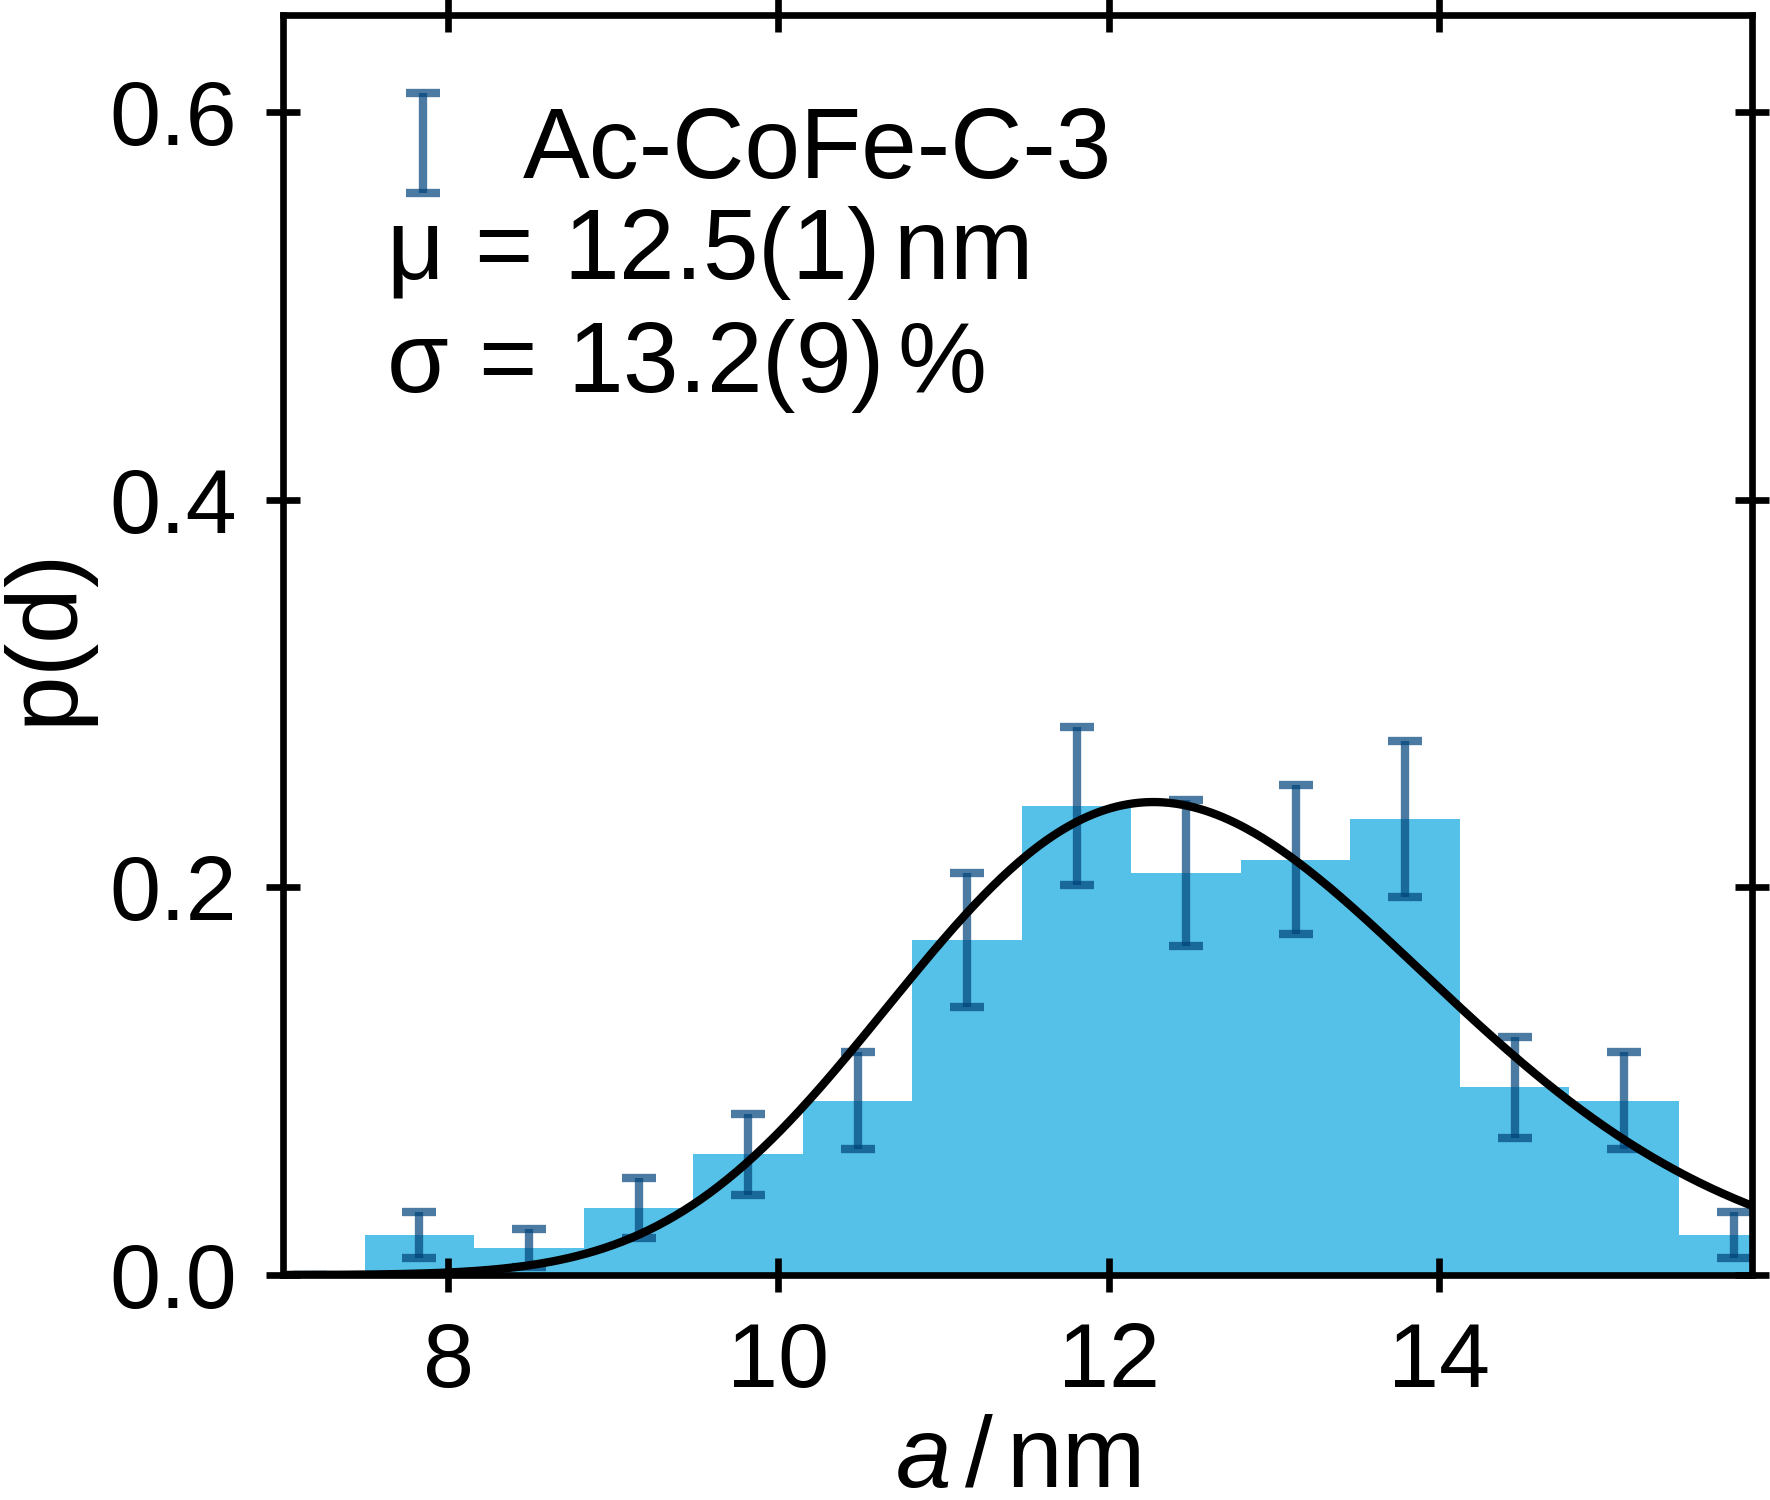
\includegraphics{monolayers_TEM_Ac_CoFe_C_3_sizeDist}
    \caption{\label{fig:monolayers:nanoparticle:tem2}Micrographs (left) and evaluated size distribution (right) of Ac-CoFe-C-3 from bright-field TEM.}
  \end{figure}

  \begin{table}[ht]
    \centering
    \caption{\label{tab:monolayers:nanoparticles:discussion:tem}Size and size distribution of the four nanocube batches as determined by TEM.}
    \begin{tabular}{ l | r | r | r | r}
      \textbf{TEM} & \textbf{Ol-CoFe-C} & \textbf{Ac-CoFe-C} & \textbf{Ac-CoFe-C-2} & \textbf{Ac-CoFe-C-3}\\
      \hline
      $\bar{a} \, / \unit{nm}$    & 10.9(1) & 10.1(1) & 10.8(1) & 12.5(1)\\
      $\sigma_{a}\, / \unit{\%}$  & 8.8(3)  & 13.9(9) & 9.9(8)  & 13.2(9) \\
      \hline
    \end{tabular}
  \end{table}
\end{document}